\chapter{Methods}\label{chap:methods}
\section{Workflow of Visualization of Network}
Below is the sequence of steps that I followed during the implementation. For this I have used python with Keras. 
\begin{figure}[h]
    \centering
    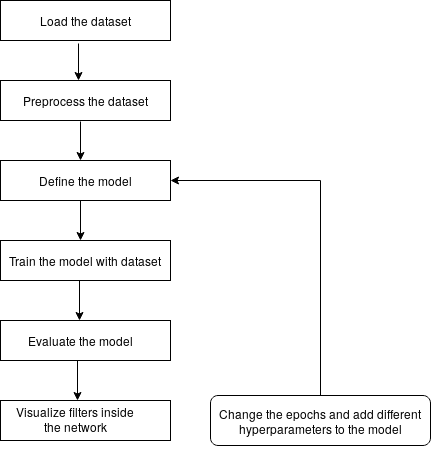
\includegraphics[width=0.7\textwidth]{thesis_template/images/flo.png}
    \caption{\small Flowchart representing steps followed}
    \label{}
    \end{figure}


\newpage \noindent \textbf{Reason to choose Keras}\\
 Keras\footnote{\url{https://keras.io/}} is an API which is built on top many other frameworks like Tensorflow, Theano and CNTK. This framework makes it easy to build bigger deep learning models with many layers with less time. It also has many pre-defined parameters and hyper parameters so we need not define each and everything in detail. 

And most importantly the main part of this work is to visualize the filters inside the model and Keras-vis\footnote{\Url{https://raghakot.github.io/keras-vis/vis.visualization/}} is used for this, so keras was used to build the models. As keras is built on the top of tensorflow later on we can also convert it into tensorflow model if needed. Finally my experience was I was able to apply many different optimizers and activation functions without any difficulty. And I got time to build and experiment on many different models.\\
PS: I have not described all the models in this section.

\subsection{Loading the dataset}
 
The dataset is MNIST which was introduced by Yann LeCun, Corinna Cortes and Christopher Burges \cite{LeCun}. It is a dataset that contains hand written digits which is a subset of larger dataset from NIST. The dataset must always be divided in to train and test dataset in order to train the model on training images and then evaluate its ability of image classification on test set. MNIST already has 60000 train images and 10000 test images which are of size $28\times28$ and are gray scale images i.e.,only one channel. Which means the height and width of an image is 28 and depth is 1. 
 
\noindent In keras it is very easy to download the dataset as it comes with a library of datasets. It has data which is already split in to train and test data and once we load the dataset X\_train, y\_train, X\_test, y\_test are loaded where X indicates images of train and test data and y indicates respective labels.

In order to go to the next step we need to have a clear understanding of the dataset. Using plot method we can look at the images to check if the data is correct. 
\begin{figure}[h]
    \centering
    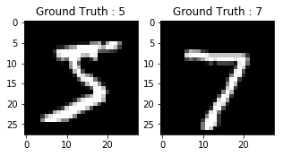
\includegraphics[width=0.5\textwidth]{thesis_template/images/screenshot.png}
    \caption{\small Random images from the dataset}
    \label{}
    \end{figure}
    
 
\newpage \section{Preprocessing the data}

This is the main step in training the model with the data because we need to convert the data in such a way that model can extract features from it. 
\subsection{Reshaping the data}
From above image it is clear that the images are in grayscale that have pixel values in the range of 0 to 255.
The data have $ 28\times28 $ dimensions hence it should be reshaped in to the form of (28,28,1) in order to feed it to the network. 

Here Tensorflow is the backend therefore the channels come last. In case of Theano the channels come first. We need to be very careful in the image dimension ordering before feeding the data to the model otherwise the model cannot take the data.


\noindent As Convolution2D layer in Keras accepts an input of 4D tensor with shape (batch, height, width, channels) if data format is "channels\_last". In this case this is done by  X\_train.reshape(-1,28,28,1), here -1 indicates that the batch size can vary. 

\subsection{Rescaling the pixel values}

In order to reduce the computational complexity we need to rescale the pixel values of the images in dataset. The pixel values range from 0 to 255 where 0 is black and 255 is white. Since 255 is the maximum value we need to divide the images by 255 so that the resulting pixels are in the range [0,1]. 
\newpage\noindent We do this in order to normalize the image values because some images have high pixel values and some have very low pixel values. Normalizing the input values to the same range lets all the images contribute evenly to the total loss as all the images in the dataset are sharing the same model and same weights. Without scaling it will be hard for the model during training to update the weights.

Scaling the pictures in same range of [0,1] helps us using only one learning rate, otherwise higher pixel values need smaller learning rates and lower pixel values need larger learning rates. Since the dataset I used has small dimensions of $28\times28$ rescaling is done by dividing it with 255, for images with higher resolution the values might vary. There is also one more thing we need to consider here the data we have is in uint8 format, now we have to convert it to "float32" format.

\subsection{One-hot encoding of labels}

Convnet model cannot operate directly on the labels of the images so we use one-hot coding to convert this categorical data in to a numerical form. It means we are creating dummy variables from categorical data. Here one-hot encoding will be a row vector of $ 1\times10 $ dimension.

 It means that the vector consists of all zeroes except for the class it represents. For example an image of class 1 has a label of [1 0 0 0 0 0 0 0 0 0].
\subsection{Splitting the training set} 
Now we have training data and testing data which is preprocessed in such a way that CNN can accept and learn from it. But there is one more vital step that is to split the training data properly in to training and validation data. Basically this is done to reduce overfitting and increase the generalization ability of the model. It can be split in to 80\% training data and 20\% validation data so that we can validate the model on the data which it has never seen before, doing this also helps in efficient performance on test data. Let us now take a look at how our data looks.


Here we have 48000 training images and 12000 validation images of shape (28,28,1)
\section{Defining the model}
This involves defining a basic model with just Convolution,relu and pooling layers. No extra regularization techniques were used here.
This step involves creating a model. Building a machine learning properly plays an important role in image classification. The structure of the model determines the performance of it. The beauty of this Convnet is we can model it according to our wish i.e., we can put as many hidden layers as we wish. In order to answer the problem statement just need few hidden layers are needed so the model is not so deep.
The model is Sequential stack of layers. I have used four Convolutional layers.
\begin{itemize}
    \item \textit{\textbf{First Convolutional layer}} will have 16 number of filters with the size of $3\times3$ which takes the input of size (28,28,1)
    \item \textit{\textbf{Second Convolutional layer}} will have 32 number of filters of same size as first layer.
    \item \textit{\textbf{Third Convolutional layer}} will have 64 number of filters of same size as previous layers.
    \item \textit{\textbf{Fourth Convolutional layer}} will have 128 number of filters of size $3\times3$ 
    \end{itemize}
\textbf{\textit{Why increasing number of filters? }}\\
The pattern of selecting the number of filters in each convolutional layer is similar to vgg16 model which has even and increasing number of filters. The layers have increasing number of filters as we go deep in to the network in order to increase the representational power of the network. Second reason is in convnets we downsample the images as we go through the network to tolerate this resolutional loss we increase the number of units. 
 \textbf{\textit{What does every convolutional layer consist of? }}\\
 Every Convolutional layer two very important hyper parameters i.e., padding and stride values. The importance of these two is explained in the Introduction. Keras can understand zero padding as "\textit{padding = same}" and with a stride of 1. \\
  PS: The most important thing observed here is when padding was not included in the convolutional layer the input got shrunk within three layers and it went in to negative values. This resulted in very shallow model and in turn the accuracy was effected. So padding is a very important hyper parameter especially when images are of low resolution. \\
  In addition to these convolutional layers there are also Relu and Max-pooling layers after each Convolution layer. Sequentially it has convolution layer followed by Relu layer followed by Max-pooling layer of size $2\times 2$.\\
  $$Conv2D\rightarrow Relu \rightarrow Maxpooling$$
  
\subsubsection{\textbf{\textit{Why only ReLU activation layer? }}}

Relu is selected over other activation functions because it is always either positive or zero but not negative. Both the activation function and its derivative is monotonic. This makes the computation cheap and helps the network converge faster without effecting the accuracy.
 \begin{figure}[h]
    \centering
    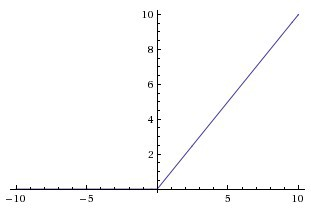
\includegraphics[width=0.5\textwidth]{thesis_template/images/rElu.jpg}
    \caption{\small Relu graph}
    \label{}
    \source{\url{https://medium.com/the-theory-of-everything/understanding-activation-functions-in-neural-networks}}
    \end{figure} 

\noindent The range of ReLU activation is [0,$\infty$). The graph of ReLu looks like linear but it is generally non-linear in nature.  And one more reason to use this function is to overcome the problem of \textit{Vanishing Gradient} which occurs especially when we use gradient based optimization methods.
\\ \textbf{ \textit{Vanishing Gradient problem:}} Convnets basically suffer from the problem of decreasing gradients when we are using more complex data like images. Now during the training process of a large networks using back-propagation the model calculates gradients of loss with respect to each trainable parameter and as we move backward the magnitude of gradients gets exponentially smaller and can also vanish completely. This happens when the activation function squashes the input in to a very small output range (0,1) and you further multiply it by even smaller learning rate. This in turn effects the value of delta to be updated and lower layers will get little or no updates. If there is a small update then the network would require larger training time and when there is no update the network cannot converge at all. The diminishing of this gradient values is referred to as vanishing gradient problem. When we use activations like sigmoid or tanh this occurs. According to \cite{Ide} the smarter and easier way to overcome this problem is by using the Relu activation as it is always positive and maps only the maximum value.\\ 

\noindent After the four convolutional, relu and pooling layers the model had two fully-connected layer followed by softmax layer.

\subsection{Compiling the model}
The model is ready now, next we have to train it using the preprocessed data. For that first we need to compile the model using the loss function and the optimizer. To compile the model we need to consider three parameters i.e., loss function, optimizer and metrics. \\
 \textbf{Loss Function:}
Here "Cross entropy" is the loss function I have used instead of Mean square error since it is already defined in Keras we can just import it. The binary cross entropy is defined by the following formula\\$$H(p,q) = -\sum_{x}p(x)log q(x) $$ \\
Here probabilities are represented by 'q' and labels are in 'p' slot. In case of CNNs and for problems like classification this loss function is more used because the output of the model is probability distribution (output layer in the model is softmax which is a set of probabilities). The lower value of this loss function indicates that the model is performing better.\\
\textbf{Optimizer:}The optimizer controls the learning rate of the parameters. The learning rate determines how fast the optimal weights for the model are calculated. Adaptive Moment Estimation(Adam) \cite{Diederik} optimization method is used here which is an extension of RMSProp optimization algorithm with momentum. \\
\noindent\textbf{\textit{Adam}} uses two tricks which makes the network to converge faster. \cite{Diederik} They are \begin{itemize}
    \item Momentum: It means that some fraction of previous update is added to current update in a way that repeated updates in one direction compound. There is no need to add momentum as a hyper parameter like in SGD as adam already incorporates it.
    \item Adaptive learning rate: It means that it uses learning rate according to the parameter. This is beneficial because the parameters in the early layers need higher learning rates and it makes sense to increase learning rates only for those parameters. This speeds up the learning. And the learning rate does not need manual tuning in this algorithm. 
\end{itemize}
For every weight $w^j$ adam calculates
$$ v_t = \beta_1 * v_{t-1} - (1- \beta_1)* g_t $$
$$ s_t = \beta_2 * s_{t-1} - (1- \beta_2) * g_t^2 $$
$$ \Delta w_t = -\eta \frac{v_t}{\sqrt{s_t + \epsilon}} * g_t $$
$$ w_{t+1} = w_t + \Delta w_t $$
Here $\eta $ is learning rate, $g_t$ gradient at time t, $v_t$ and $g_t$ are exponential averages of gradient and gradient squares respectively. The parameters $\beta_1 $ and $\beta_2$ are exponential decay rates of first and second moments respectively. We used standard values of these two parameters as proposed by the authors i.e., 0.9 for $\beta_1$ and 0.999 for $\beta_2$. And the other parameter is learning rate or the size of step which has very small value. \cite{Diederik} \\
\noindent\textit{\textbf{Why is Adam better than SGD?}} \\
SGD maintains a single learning rate throughout the training process but Adam computes  individual adaptive learning rates for each parameter from estimates of both first and second moments of the gradients. It means it does not adapt learning rates just based on first momentum but also considers the average of second momentum. Adam learns the learning rate itself on per-parameter basis. 



\section{Training the model}
Now we have both data and the model now its time to train the network. To train the network here we use 'fit()' function on our model with different parameters like training data X\_data and validation data along with batch size and number of epochs it should be trained. 


\noindent In order to visualize the performance of the model during the training process after each epoch we define history. The batch-size and the number of epochs can be changed and they have huge effect on the accuracy and performance of the model. It means that more number of times we pass the data through the network more accurate it will perform. 
While doing this we can see the training and validation accuracy and loss of the model. Next we can test this machine learning model by using it to make predictions on test data(model.predict() method is used for this).\\ 
  But accuracy alone is not enough to evaluate the model. Because it hides the details we need to better understand the performance of our model. Especially when we are dealing with multi-class classification we need to know if the images are predicted correctly or not, for this we need to validate our model's performance using precision, recall and F1 scores. The detailed explanation for these metrics is described in the next section.


\section{Evaluation of model using different metrics}
\subsection{Confusion-Matrix}
\textit{What is confusion matrix?}\\
As the name suggests it is a matrix that tells how many times your model was confused while making predictions. It gives the deeper intuition on the performance of any machine learning model. The matrix helps you determine what are the categories that you often get right and much more importantly, which are the ones you often get wrong. To understand confusion-matrix and other metrics which are described in further sections we need to understand these terms \textit{true positives,true negatives, false positives and false negatives.} \cite{inproceedings}
\begin{itemize}
    \item \textbf{True Positive(TP):} The model predicted positive and it is true.
    \item \textbf{True Negative(TN):} The model predicted negative and it is true.
    \item \textbf{False positive(FP):} The model predicted negative but it is true.
    \item \textbf{False Negative(FN):} The model predicted negative and it is false.
    \end{itemize}

The matrix consists of these values. For example a basic binary classifier has a confusion-matrix that has these values as follows.
\begin{figure}[h]
    \centering
    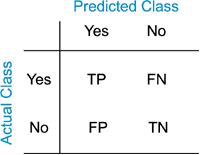
\includegraphics[width=0.4\textwidth]{thesis_template/images/con1.png}
    \caption{\small Confusion-matrix}
    \label{}
    \source{\url{https://en.wikipedia.org/wiki}}
    \end{figure}\\
The matrix has
\begin{itemize}
    \item Rows: Which represent the actual class.
    \item Columns: Which correspond to the predicted class.
\end{itemize}
\noindent In a multi-class classification model confusion-matrix gives a clear visualization of how many images in the dataset are predicted correctly. To calculate this we need a validation dataset with expected outputs. 
 The number of correct and incorrect classifications are filled in the table. The total count of correct predictions for a class go in to the expected row and predicted column for that respective class. In this case the model is trained on 10 different class and achieved accuracy of 99.8\% on test dataset. To calculate confusion-matrix Skicit learn library is used. 


 \subsection{Precision, Recall and F1-score}
 
\textit{\textbf{Precision}} also called Positive Predictive value is the ratio of number of True Positives predicted by the model to number of True Positives and false positives. 
$$ Precision = \frac{TP}{TP+FP}$$
This score tells us how precise our model had made classifications and for every class how much it predicted correctly. It should be as high as possible. \\

\noindent \textit{\textbf{Recall}} also called as Sensitivity or True Positive Rate is the number of True Positives divided by the number of True Positives and number of False Negatives. 
$$ Recall = \frac{TP}{TP+FN}$$
So it can be understood as a measure of classifiers completeness. The value should be as high as possible otherwise it indicates many False Negatives.

\noindent \textit{\textbf{F1-Score}} is the harmonic mean of Precision and Recall. It takes both False Positives and False Negatives in to account. It uses harmonic mean instead of arithmetic mean by punishing extreme values more. It is difficult to compare two models with low Precision and high recall or vice versa. So to make them comparable we use F1-score. It measures both metrics at the same time.
$$F1 = 2* \frac{Precision*Recall}{Precision+Recall} $$

\noindent F1-score is more useful than accuracy of the model as it considers both False Positives and False Negatives. \cite{scikit-learn}







\subsection{AUC-ROC Curve}
Another most popular metric is ROC which is Receiver Operating Characteristic curve which helps us in visualizing the performance of a machine learning model. An ROC curve plots true positive rate(TPR) on the y-axis versus false positive rate(FPR) on the x-axis. It shows how the TPR and FPR values vary as we modify the threshold for identifying a positive in our model. The value of threshold is changeable.

\noindent Here TPR is Recall. To understand FPR we need to know Specificity which is 
$$ Specificity = \frac{TN}{TN+FP} $$
$$ FPR = 1 - Specificity$$

\noindent AUC means Area Under Curve which represents the measure of seperability. It gives us an intuition about how much the model is able to distinguish between diferrent classes. By calculating AUC we can quantify the model's ROC curve \cite{Yang}. All these performance metrics obtained for this model are shown in the results section.
 


\section{Visualizing the filters inside the network}
The first important thing is the method involves visualizing convolutional layers, fully-connected layers are not included. Keras makes it easy to save and load the model, this avoids training it multiple times and saving time.

 \subsection{Visualizing by Activation Maximization} The first method is finding the input image that maximizes the activation of a filter. It is an activation based method. The idea is that every filter is capable of learning different patterns from the input image and we need to generate an image that produces high output activation for that filter. Keras-vis library is used for this which has $visualize\_activation$ API to visualize activations of the filter. The method is known as activation maximization \footnote{\url{https://raghakot.github.io/keras-vis/visualizations/activation_maximization/}} and it calculates $$ \frac{\partial ActivationMaximization Loss}{\partial input}$$ 
Before proceeding further keras-vis should be installed. Now we need to know the layer names of each layer to make it easy for us to know which layer we want to visualize and model.summary() provides this facility. It gives us the clear picture of name and number of parameters in that layer. For this use case we need to use visualize\_activation to look at what filters are recognizing. 

 \noindent The most important thing to understand about this method is that filters and output are kept constant and input is modified so that it maximizes certain units in the model. First activation layer was chosen to visualize which has name 'activation\_1'. For this method layer\_idx and filter\_indices are the important arguments where layer\_idx indicates the index of layer that need to be visualized and filter\_indices refer to the index of filter in the  layer. Here layer\_idx is set to convolution layer. 

\begin{figure}[h]
    \centering
    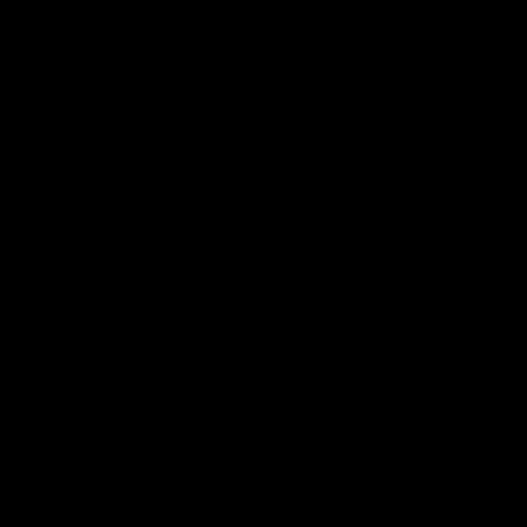
\includegraphics[width=0.6\textwidth]{thesis_template/images/stitchedfilter.png}
    \caption{\small stitched filters of first activation layer}
    \label{}
    \end{figure}

\noindent By using this method on first activation layer it gave the output which was totally black. The image below represents the outcome of this method. For different layer\_idx and different images it gave the same outcome. 

\newpage \noindent This is the reason why next method was taken in to consideration. It is visualizing the filters of individual layers. This is possible by defining a method for plotting the filters. 

 \subsection{Visualization of Intermediate layers}

Here comes the interesting part of this work, to achieve first layer visualizations we have to define a function which takes one argument which is layer name\footnote{\url{http://cs231n.github.io/understanding-cnn/}}. This method made it easy to visualize the filters inside each layer given particular image. For this random images can be chosen from the test dataset and then visualize the features of that image in the network.
 To understand more clearly this model has 32 filters in the first layer. Hence for the image generated randomly there were 32 different activations where each activated filter was again an image. 
 
 
 The outcome of this experiment is discussed in the results section. In addition to this the section consists of the visualizations of slightly modified model with different parameters.  



    